%\documentclass[tikz, border=5pt]{standalone}
\begin{document}
	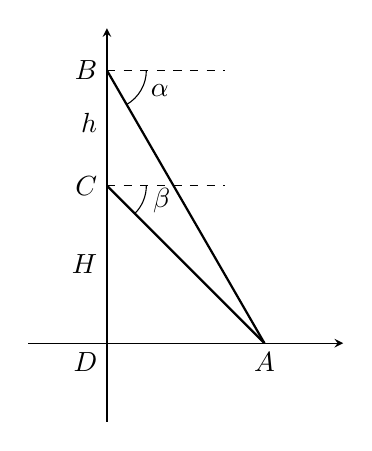
\begin{tikzpicture}[>=stealth, scale=1]
		% 绘制坐标轴
		\draw[->] (-1,0) -- (3,0) ; % x轴(带箭头和标签)node[below] {$x$}
		\draw[->] (0,-1) -- (0,4) ; % y轴(带箭头和标签)node[below left] {$y$}
		\node at (0,0) [below left] {$D$};           % 原点O的标签
		
		% 直线
		\draw[thick] (2, 0) -- (0, 2) ; 
		\draw[thick] (2, 0) -- ++(120:4) ; 
		
		% 绘制虚线辅助线
		\draw[dashed] (0,{2*tan(60)}) -- (1.5,{2*tan(60)});  % B的虚线
		\draw[dashed] (0,2) -- (1.5,2);  % C的虚线
		
		% 标记各点的标签
		\node at (2,0) [below] {$A$};
		\node at (0,2) [ left] {$C$};
		\node at (0,{2*tan(60)}) [ left] {$B$};
		
		\node at (0,1) [left] {$H$};
		\node at (0,2.8)  [left] {$h$};
		
		%  弧线
		\draw (0.5, {2*tan(60)}) arc (0:-60:0.5) node[midway, right] {$\alpha$}; 
		\draw (0.5, 2) arc (0:-45:0.5) node[midway, right] {$\beta$}; 
		
	\end{tikzpicture}
\end{document}
